\documentclass[12pt,a4paper]{article}

%%% REPORT FOR SPIN WAVES EXCITATION BY ACOUSTIC PULSE

\usepackage{amsmath}               %AMSMath tools for flexible equations
\usepackage[english]{babel}
\usepackage{graphicx}
\usepackage{cite}
%\usepackage[margin=1.5cm]{geometry}
\usepackage{fullpage}   % Texte en pleine page, réduction des marges 
\usepackage{subfig} % remplace subfigure
%\usepackage[utf8x]{inputenc} 
\usepackage[latin1]{inputenc} 
\usepackage[T1]{fontenc} 
\usepackage[section]{placeins}
\usepackage{listings} % in order to include code in a tex file
\usepackage{setspace}
\onehalfspacing
\usepackage{hyperref}


%\renewcommand{\thefootnote}{\fnsymbol{footnote}}
\renewcommand{\thefootnote}{\arabic{footnote}}
\DeclareTextSymbol{\degre}{T1}{6}

\newcommand{\valentin}{\textbf{Valentin}}
\newcommand{\vladimir}{\textbf{Vladimir}}
\newcommand{\anton}{\textbf{Anton}}
\newcommand{\alexandr}{\textbf{Alexandr}}
\newcommand{\vasily}{\textbf{Vasily}}
\newcommand{\dmitrii}{\textbf{Dmitrii}}
	
\begin{document}
	
	
\begin{center}
	{\bf\Large Meeting Recap~\MakeUppercase{\romannumeral 16}}\\
	{\bf\Large \today}\\
	\vspace{0.4cm}
	{\large Valentin \textsc{Besse}\footnote{Author of the report}, Vladimir \textsc{Vlasov}, Anton \textsc{Golov}, Alexandr \textsc{Alekhin}, Dmitrii \textsc{Kuzmin} and Vasily \textsc{Temnov}}\\
	\vspace{0.6cm}
	%{\large \today}
	%{\large August 28, 2017}
\end{center}
\vspace{0.1cm}

\section*{Version}

\begin{itemize}
    \item February 20, 2018: V1.
\end{itemize}

\section*{Present at the meeting}

\begin{itemize}
    \item Valentin \textsc{Besse}.
    \item Vladimir \textsc{Vlasov}.
    \item Anton \textsc{Golov}.
    %\item Alexandr \textsc{Alekhin}.
    %\item Dmitrii \textsc{Kuzmin}.
    %\item Vasily \textsc{Temnov}.
\end{itemize}

\section*{Agenda}

During this meeting we discuss about:
\begin{enumerate}
    \item Implementation of non-zero initial condition (see Sec. \ref{sec1}).
    \item Influence of strain's front to exchange interaction (see Sec. \ref{sec2})
    \item Travel of Valentin to Syktyvkar after Saint-Petersburg Symposium (see Sec. \ref{sec3})
\end{enumerate}

\section{Implementation of non-zero initial condition}
\label{sec1}
\anton\ shows illustration of non-zero initial condition that he can use to study the impact of strain's dependence of the exchange interaction on spin wave dynamics (see Fig. \ref{fig:NonZeroIntialCondition}).
\begin{figure}
    \centering
    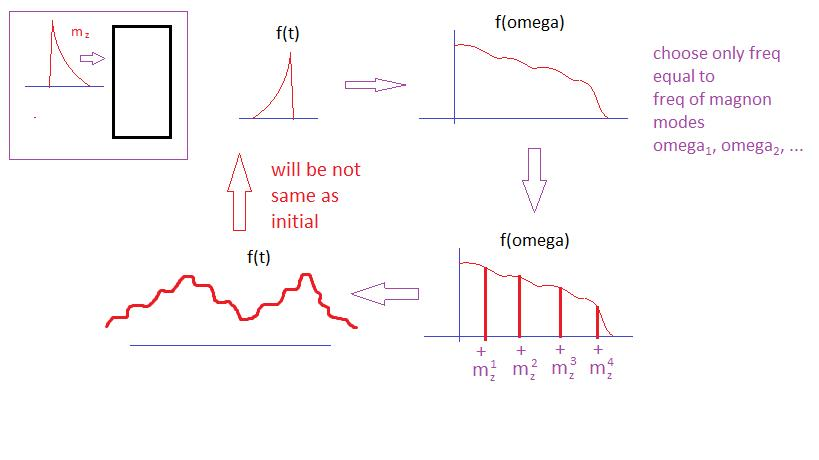
\includegraphics[width=\textwidth]{idea_exchange_from_initial_m_not_zero.png}
    \caption{Anton's illustration of non-zero initial condition.}
    \label{fig:NonZeroIntialCondition}
\end{figure}
\anton\ will design the non-zero initial condition and he will keep only the magnons frequencies.
\anton\ will do the simulations and present his result next Tuesday (March 6th).

\section{Influence of strain's front to exchange interaction}
\label{sec2}
Since we use an integral approximation to the strain dependence in our system of equations, \vladimir\ explains that our model does not include the influence of the strain's front (exception when the strain enters or exits the film).
\vladimir\ suggests that we have a reflection on how could we include this effect in our model.

\section{Travel of Valentin to Syktyvkar}
\label{sec3}
\vladimir\ proposes to \valentin\ to go to Syktyvkar after Saint-Petersburg Symposium.
\valentin may arrive to Saint-Petersburg on Sunday June, 3rd and leave on Saturday June, 9th (or Sunday June 10th).
\vladimir\ proposes that Syktyvkar pay for \valentin's\ hotel and food expense.
\valentin\ will leave Syktyvkar on Saturday June, 16th.

\valentin\ want to discuss this \vasily.

Also \valentin may have an issue with his arrival to Saint-Petersburg because the audition for Maitre De Conference's position will be at the end of May (and maybe at the beginning of June).

\section{New tasks}

The new tasks are:
\begin{itemize}
    \item Simulation and study of the impact of strain's dependence of the exchange interaction on spin wave dynamics.
\end{itemize}

\section*{Next meeting}

The next meeting will be \textbf{Tuesday March 6th at 11:30 am (CET)}.

\newpage

\section*{List of abbreviations}

\begin{table}[ht]
    %\centering
    \begin{tabular}{ l c r }
        Landau-Lifschitz-Gilbert & $\Longrightarrow$ & LLG \\
        Ferromagnetic resonance & $\Longrightarrow$ & FMR \\
    \end{tabular}
\end{table}

%\bibliographystyle{ieeetr}
%\bibliography{Exchange_Magnons}

\end{document}